\documentclass[tikz,border=6pt]{standalone}
\usepackage{amsmath,amssymb}
\usepackage{tikz}
\usetikzlibrary{decorations.pathmorphing, decorations.markings, arrows.meta}
\begin{document}
% ▼▼▼【参数调节区】▼▼▼
% scale: 整体大小 (1.5 倍)
% line width: 线条粗细 (1pt)
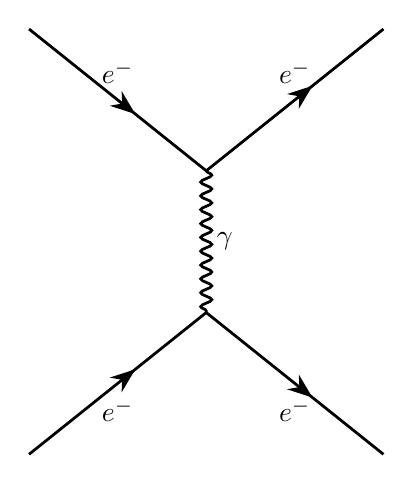
\begin{tikzpicture}[scale=1.5, line width=1pt,
    % 样式定义
    photon/.style={decorate, decoration={snake, amplitude=2pt, segment length=5pt}},
    fermion/.style={postaction={decorate},
        decoration={markings,mark=at position 0.6 with {\arrow{Stealth[scale=1.2]}}}}
]

    % ▼▼▼【坐标调节区 - 这里的数值决定了"折角"的大小】▼▼▼
    
    % --- 上半部分 (Top) ---
    % 入射点 (左上，Y=1.8) -> 撞击点 (中间，Y=0.6) -> 出射点 (右上，Y=1.8)
    % 注意：1.8 和 0.6 的差距越大，折角越明显！
    \coordinate (in_top)    at (-1.5,  1.8); 
    \coordinate (v_top)     at (0,     0.6);   
    \coordinate (out_top)   at (1.5,   1.8);  

    % --- 下半部分 (Bottom) ---
    % 入射点 (左下，Y=-1.8) -> 撞击点 (中间，Y=-0.6) -> 出射点 (右下，Y=-1.8)
    \coordinate (in_bottom) at (-1.5, -1.8); 
    \coordinate (v_bottom)  at (0,    -0.6);   
    \coordinate (out_bottom) at (1.5, -1.8);  

    % ▼▼▼【连线区】▼▼▼
    
    % 上路电子 (折线)
    \draw[fermion] (in_top) -- (v_top) node[midway, above=2pt] {$e^-$};
    \draw[fermion] (v_top) -- (out_top) node[midway, above=2pt] {$e^-$};
    
    % 下路电子 (折线)
    \draw[fermion] (in_bottom) -- (v_bottom) node[midway, below=2pt] {$e^-$};
    \draw[fermion] (v_bottom) -- (out_bottom) node[midway, below=2pt] {$e^-$};

    % 中间交换光子
    \draw[photon] (v_top) -- (v_bottom) node[midway, right] {$\gamma$};

\end{tikzpicture}
\end{document}
